\documentclass[tikz, border = 2pt]{standalone}

%---------------------------------------------------------------------------%
% PACKAGES                                                                  %
%---------------------------------------------------------------------------%

%----- MATH
%---------------------------------------------------------------------------%
\usepackage{amsmath, amssymb}

%----- FIGURES
%---------------------------------------------------------------------------%
\usepackage{pgfplots}
\pgfplotsset{compat=1.13}

\begin{document}

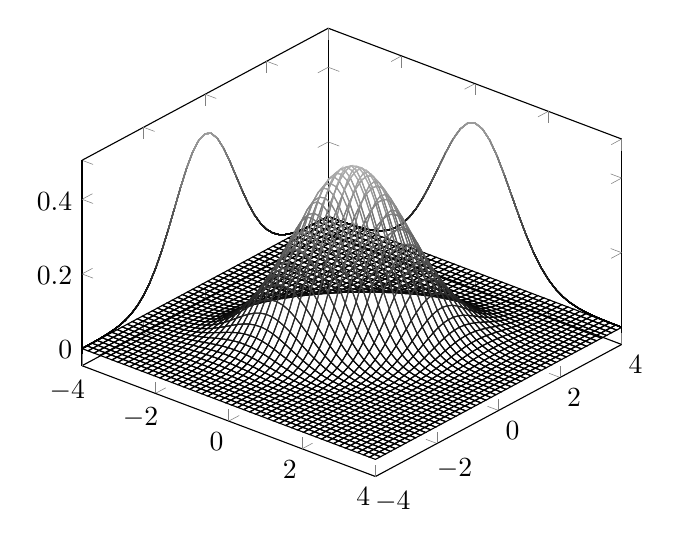
\begin{tikzpicture}
  \begin{axis}[
  colormap={}{ gray(0cm)=(0); gray(1cm)=(0.7)},
  view/h =40,
  view/v =40,
domain=-4:4,
domain y=-4:4,
]

\newcommand\expr[2]{(1/sqrt(2*pi*3/4))*exp(-(#1^2 - #1*#2 + #2^2)/(3/2))}
\newcommand\exprx[1]{(1/sqrt(2*pi))*exp(-(#1^2)/2)}

\addplot3[
samples=41,
samples y=10,
domain=-4:4,
domain y=-4:4,
% we want 1d (!) individually colored mesh segments:
mesh, patch type=line,
x filter/.code=\def\pgfmathresult{-4},
] 
(y,x,{\exprx{x}});

\addplot3[
samples=41,
samples y=10,
% we want 1d (!) individually colored mesh segments:
mesh, patch type=line,
y filter/.code=\def\pgfmathresult{4},
] 
{\exprx{x}};

\addplot3[mesh,samples=50]
{\expr{x}{y}};

\end{axis}
\end{tikzpicture}

\end{document}